\section{eo\-Functor\-Base Class Reference}
\label{classeo_functor_base}\index{eoFunctorBase@{eoFunctorBase}}
Base class for functors to get a nice hierarchy diagram.  


{\tt \#include $<$eo\-Functor.h$>$}

Inheritance diagram for eo\-Functor\-Base::\begin{figure}[H]
\begin{center}
\leavevmode
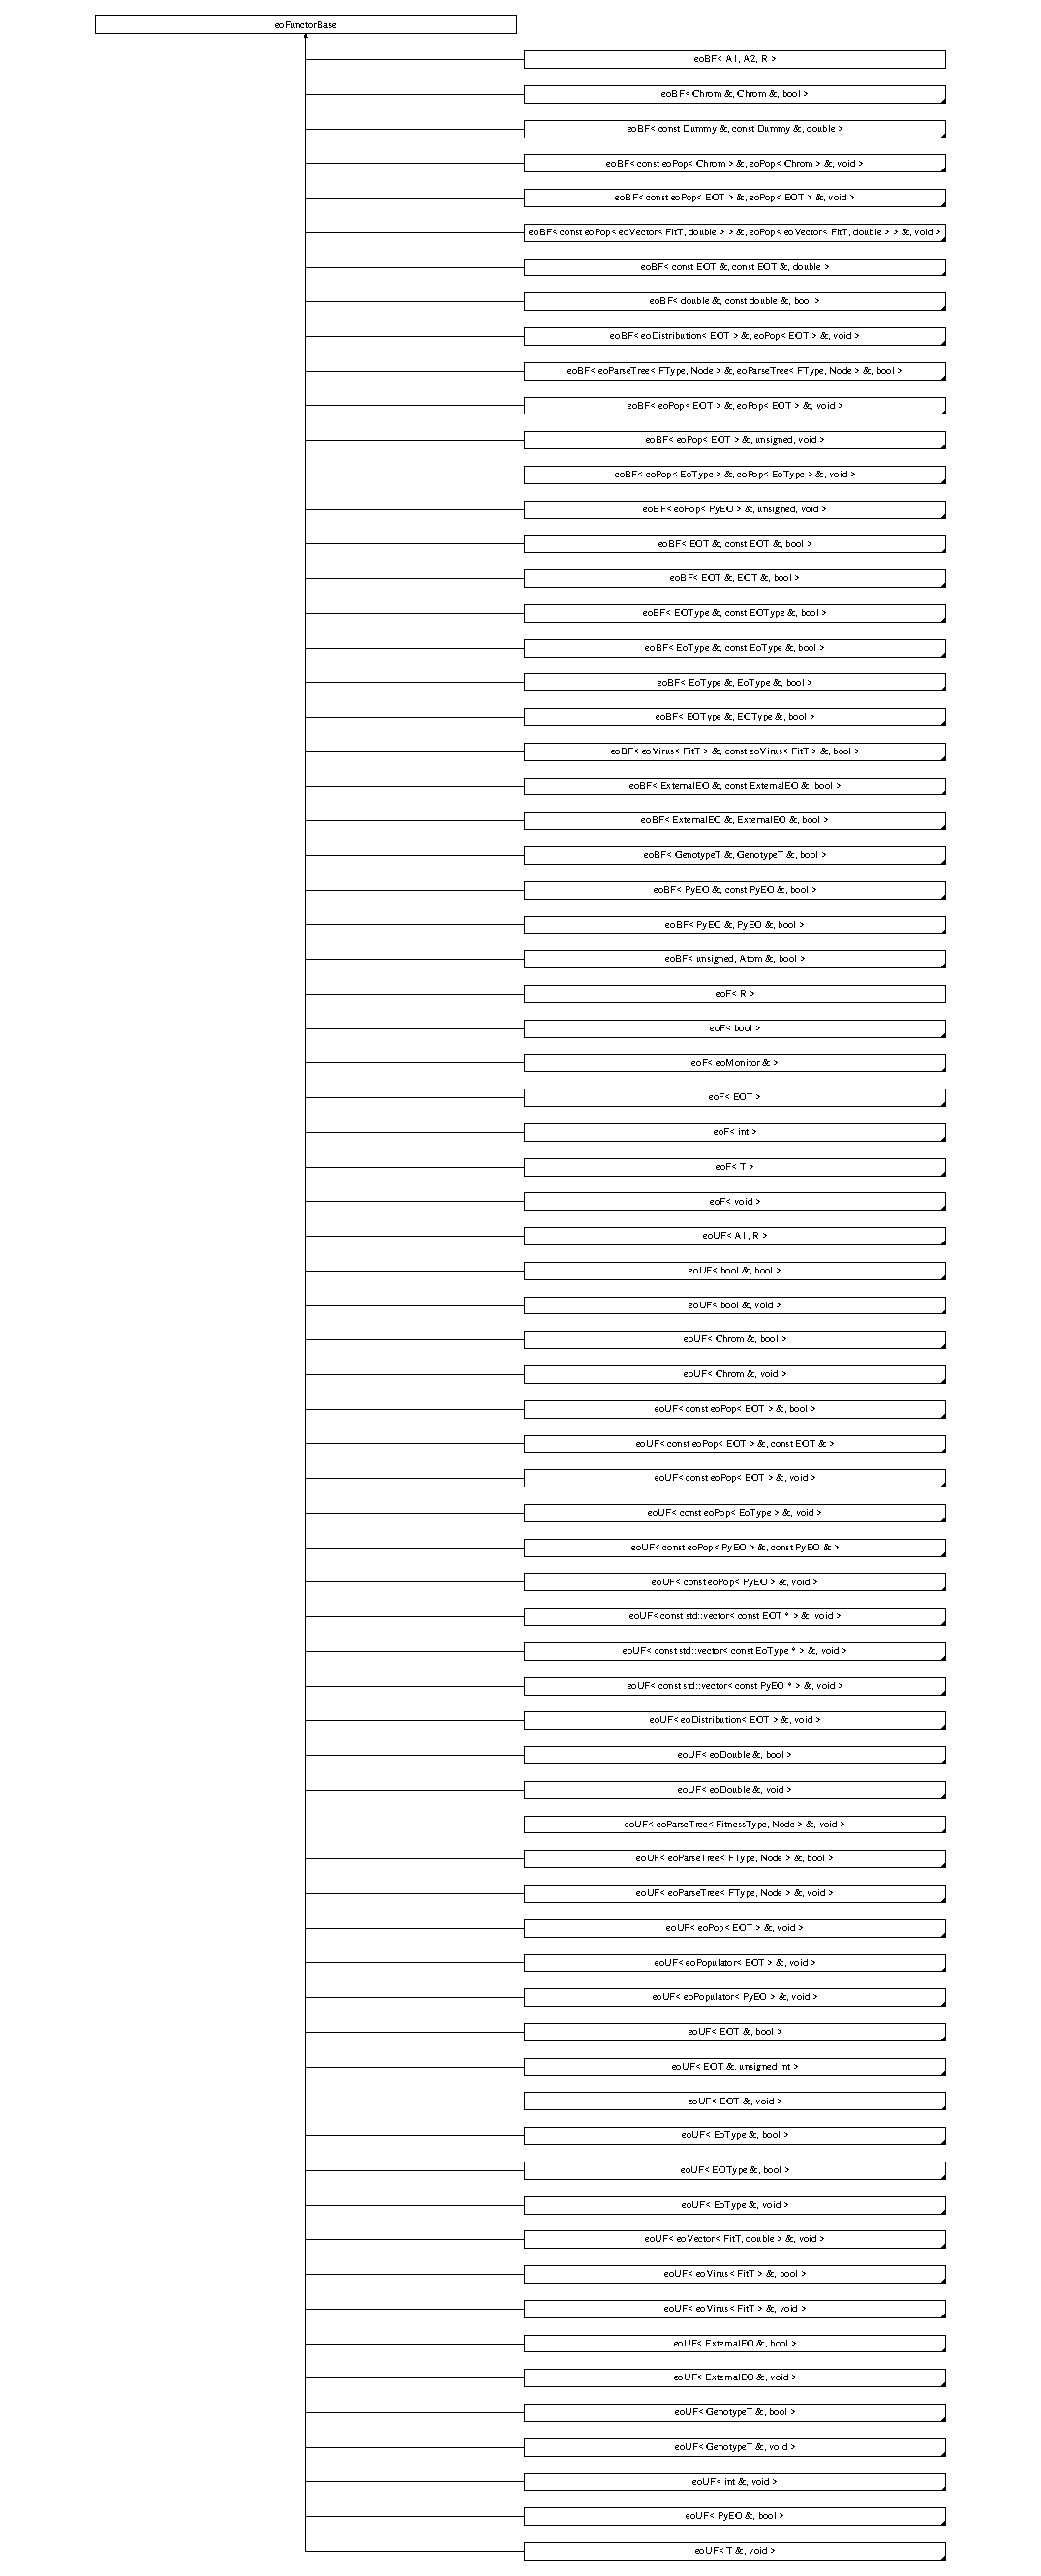
\includegraphics[height=12cm]{classeo_functor_base}
\end{center}
\end{figure}
\subsection*{Public Member Functions}
\begin{CompactItemize}
\item 
virtual {\bf $\sim$eo\-Functor\-Base} ()\label{classeo_functor_base_a0}

\begin{CompactList}\small\item\em virtual dtor here so there is no need to define it in derived classes \item\end{CompactList}\end{CompactItemize}


\subsection{Detailed Description}
Base class for functors to get a nice hierarchy diagram. 

That's actually quite an understatement as it does quite a bit more than just that. By having all functors derive from the same base class, we can do some memory management that would otherwise be very hard.

The memory management base class is called {\bf eo\-Functor\-Store}{\rm (p.\,\pageref{classeo_functor_store})}, and it supports a member add() to add a pointer to a functor. When the functor\-Store is destroyed, it will delete all those pointers. So beware: do not delete the functor\-Store before you are done with anything that might have been allocated.

\begin{Desc}
\item[See also:]{\bf eo\-Functor\-Store}{\rm (p.\,\pageref{classeo_functor_store})} \end{Desc}




Definition at line 46 of file eo\-Functor.h.

The documentation for this class was generated from the following file:\begin{CompactItemize}
\item 
eo\-Functor.h\end{CompactItemize}
